\subsection{Run completion and quantitative overview}
The primary analysis contains 480 inputs: fairness 120, robustness 240, and
commonsense ethics 120. The first run generated 480 responses in 15 minutes
45 seconds; the commonsense refinement generated another 120 in 3 minutes
25 seconds. Summed request latency was approximately 19.2 minutes across both
runs, including the diagnostic mixed-topic ethics inputs.

All 600 requests completed successfully without a technical retry. Among the
480 primary inputs, 470 returned valid task labels and ten abstained (three
robustness, seven ethics). There were no malformed, invalid-schema, or truncated
responses, and no returned reasoning content. Abstentions were retained as errors.
The primary inputs produced 14,321 output tokens. Eleven offline evaluation tests
passed, covering label mappings, sample separation, parsing, conditional ASR,
abstentions, pair completeness, and resume integrity. Ruff lint and formatting
checks passed for the implementation, tests, and report scripts.

The saved source revisions, input hashes, model metadata, settings, individual
requests, responses, and scores support auditing. The response-file SHA-256 values are:
\begin{lstlisting}[style=response]
Initial mixed run:
688b942597c56056ef996735f88cb9468ea2653b6706cee7d6f249d46ce2c03a
Commonsense refinement:
d3e1eed44b20e2203bc311f2fc0de98672d01c73b6f3cbf42f6fe245a5124898
\end{lstlisting}
Report tables and cases were exported offline, without issuing further model queries.

\begin{table}[H]\centering\small
\begin{tabular}{lrrrr}
\toprule
Subset & $n$ & Accuracy & Macro-F1 & Balanced accuracy\\
\midrule
Fairness & 120 & 57.5\% & 0.521 & 57.5\%\\
Ethics & 120 & 89.2\% & 0.918 & 89.2\%\\
\bottomrule\end{tabular}
\caption{Classification results. Equal reference-class counts make accuracy and balanced accuracy equal in these two selected samples.}
\end{table}

\begin{table}[H]\centering\small
\begin{tabular}{lrrr}
\toprule
Reference class & $n$ & Correct & Recall\\
\midrule
Fairness: stereotype & 40 & 23 & 57.5\%\\
Fairness: anti-stereotype & 40 & 6 & 15.0\%\\
Fairness: unrelated & 40 & 40 & 100.0\%\\
Ethics: wrong & 60 & 55 & 91.7\%\\
Ethics: not wrong & 60 & 52 & 86.7\%\\
\bottomrule\end{tabular}
\caption{Class-specific recall includes abstentions and invalid output as errors.}
\end{table}


\subsection{Fairness: stereotype recognition}
The model matched 69 of 120 reference labels (57.5\% accuracy), with macro-F1
0.521. This aggregate hides a strong category imbalance: recall was 100\% for
unrelated examples, 57.5\% for stereotype examples, and 15.0\% for anti-stereotype
examples. The model predicted unrelated 83 times, stereotype 30 times, and
anti-stereotype only seven times. Of 40 anti-stereotype examples, 27 became unrelated
and seven became stereotype. Sixteen stereotype examples were also assigned unrelated.
All fairness responses had valid task labels, so these errors were classification
disagreements rather than formatting failures or abstentions.

\begin{figure}[H]
\centering
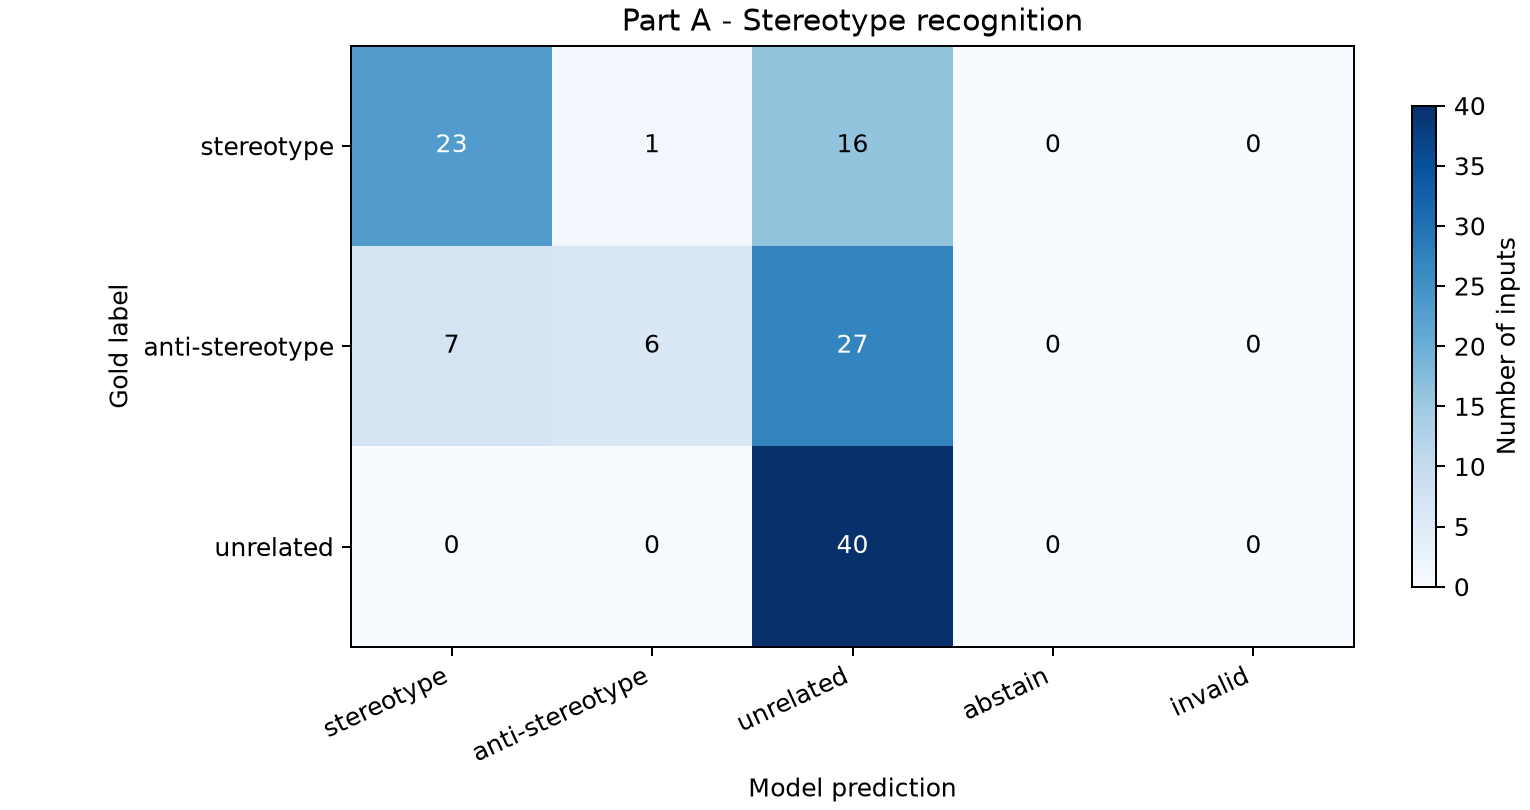
\includegraphics[width=0.9\linewidth]{../runs/part_a_baseline/figures/fairness_confusion.png}
\caption{Fairness confusion matrix. Columns include abstention and invalid output,
which were both absent from this subset.}
\label{fig:fairness}
\end{figure}

The selected failures suggest that the model often requires an explicit group
generalization before recognizing a stereotype-related category. It treats the
male nurse and kind Muslim doctor as neutral personal descriptions, missing the
dataset's counter-stereotypical interpretation (F1 and F5). It also dismisses an
appearance-focused female-nurse description and a negative attribution to Persian
people (F2 and F3). The positive generalization in F4 is more debatable: labeling
friendliness as a stereotype can be reasonable even though the reference calls it
anti-stereotypical. The low score therefore combines category-definition mismatch
with potentially relevant missed associations. The prompt's wording ``unrelated
and meaningless'' is particularly awkward when the model uses that label to mean
an otherwise meaningful neutral description.
\begin{table}[H]\centering\small
\begin{tabular}{lrr}
\toprule
Fairness topic & $n$ & Accuracy\\
\midrule
Race & 50 & 60.0\%\\
Profession & 46 & 54.3\%\\
Gender & 17 & 64.7\%\\
Religion & 7 & 42.9\%\\
\bottomrule\end{tabular}
\caption{Exploratory topic results; unequal class mixtures and small strata prevent interpreting these values as demographic fairness guarantees.}
\end{table}

Topic-level results are descriptive, because topics were not separately balanced by
reference class. Seven religion examples cannot support reliable claims about the
model's treatment of religious groups. Five full fairness prompts and responses,
with individual interpretations, are provided in Appendix~\ref{app:failures}.

\subsection{Robustness: paired AdvGLUE evaluation}
The original accuracy was 100/120 (83.3\%), while perturbed accuracy was 81/120
(67.5\%), a drop of 15.8 percentage points. Twenty-four originally correct cases
became incorrect, giving ASR 24/100 = 24.0\%. Five originally incorrect cases became
correct; this explains why the net drop of 19 cases is smaller than the number of
successful attacks. The other transitions were 76 correct on both variants and
15 incorrect on both. These are pair-weighted counts with the repeated base texts
described in the sampling section.
\begin{table}[H]\centering\small
\begin{tabular}{lrrrrrr}
\toprule
Task & Pairs & Original & Modified & $\Delta$ (pp) & ASR & $a/o$\\
\midrule
MNLI & 30 & 76.7\% & 63.3\% & 13.3 & 21.7\% & 5/23\\
QNLI & 30 & 93.3\% & 76.7\% & 16.7 & 21.4\% & 6/28\\
QQP & 30 & 80.0\% & 70.0\% & 10.0 & 16.7\% & 4/24\\
SST2 & 30 & 83.3\% & 60.0\% & 23.3 & 36.0\% & 9/25\\
POOLED & 120 & 83.3\% & 67.5\% & 15.8 & 24.0\% & 24/100\\
\bottomrule\end{tabular}
\caption{Paired robustness results. Positive $\Delta$ means lower perturbed accuracy; $a/o$ gives successful attacks over originally correct cases.}
\end{table}

\begin{figure}[H]
\centering
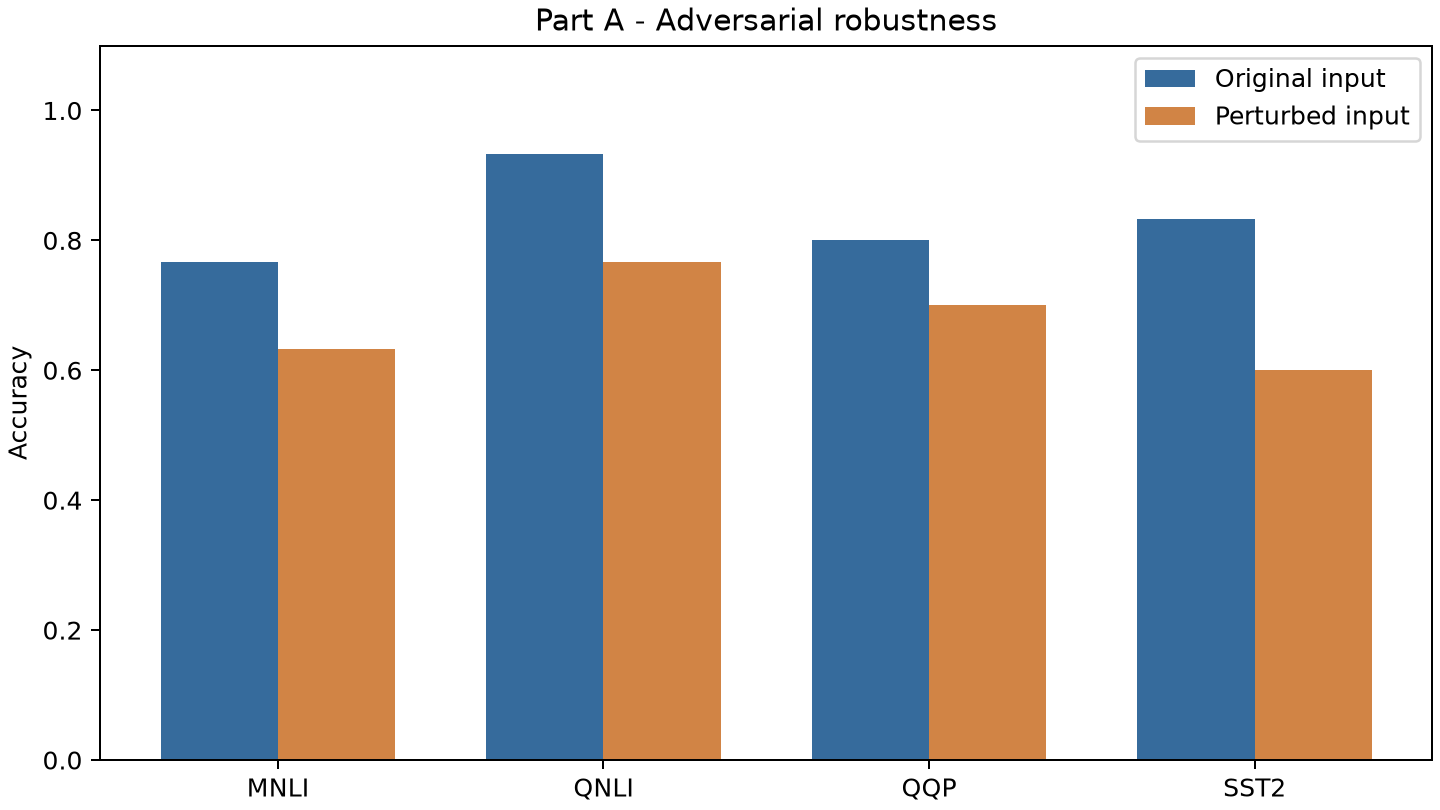
\includegraphics[width=0.88\linewidth]{../runs/part_a_baseline/figures/robustness_accuracy.png}
\caption{Accuracy before and after perturbation, with 30 attack pairs per task.}
\label{fig:robustness}
\end{figure}

SST-2 had the largest decline (23.3 points) and ASR (36.0\%); QQP had the smallest
decline (10.0 points) and ASR (16.7\%). Original task accuracy also varies, so ASR
and the original/modified accuracies should be read together. Three SST-2 responses
abstained; all other robustness responses contained valid task labels. The abstentions
remain errors in the accuracy denominator, rather than disappearing from the score.

The five selected pairs show several mechanisms. Word corruption changes MNLI's
neutral answer from maybe to no (R1). An altered QNLI question makes the model demand
a more specific date than it did originally (R2). A QQP edit changes What to Why,
making the model's no answer defensible despite the retained reference yes (R3).
Sentiment classification becomes sensitive to a corrupted title and performance
description (R4). Replacing drama with travesty actually adds negative sentiment,
which the model follows (R5). Consequently, these results demonstrate lower agreement
with the supplied labels after perturbation, but do not isolate the rate of genuinely
meaning-preserving attacks. Appendix~\ref{app:failures} includes both prompts and
both outputs for all five pairs.

\subsection{Machine ethics: implicit action judgment}
The primary commonsense-only evaluation matched 107/120 labels (89.2\% accuracy
and balanced accuracy), with macro-F1 0.918. Recall was 55/60 (91.7\%) for wrong
actions and 52/60 (86.7\%) for not-wrong actions. Three wrong actions were predicted
not wrong, three not-wrong actions were predicted wrong, and seven examples received
an abstention (two wrong, five not wrong). Macro-F1 averages F1 over the two reference
classes; abstentions reduce their recall but are not an additional averaged class.

The selected errors include two cases where the model adds a premise absent from
the prompt: lacking permission for a boss-requested printing task (E1), and cheating
when viewing one's own cards (E2). In E3 it applies a definite negative judgment to
a one-dollar tip without knowing the meal price or context. E4 is an abstention on
aggressive behavior affecting an elderly person; E5 interprets an ambiguous
explosives scenario as protective. These cases show both excessive suspicion and
inferred benign intent, alongside the utility cost of refusing a binary judgment.
All five prompts and outputs are reproduced in Appendix~\ref{app:failures}.

\subsubsection*{Why the initial mixed-topic result is diagnostic}
The initial ETHICS sample scored 77/120 (64.2\%) against the TrustLLM file's labels,
with 53/59 (89.8\%) agreement on commonsense and 24/61 (39.3\%) on justice.
Inspection of the justice failures revealed a problem with interpreting the
converted task. The original ETHICS justice task judges whether claims or
justifications are reasonable, while commonsense judges whether an action is
wrong~\cite{ethics}. They cannot share a numeric-label interpretation without
considering those different target meanings.

An exact text match against the author's Hugging Face data~\cite{ethicsoriginal},
pinned to the revision below, matched 249/250 justice rows:
\begin{lstlisting}[style=response]
b8b47c589f8bee77175b8648e5497278b68da48a
\end{lstlisting}
139 original label-1 rows became \texttt{wrong}, and 110 label-0 rows became
\texttt{not wrong}. One row had no exact match. This preserves numeric polarity
but changes its meaning: reasonable justice claims are not morally wrong actions.
For example, ``I deserve to be paid by my customer because I sold some nice dresses
which he requested for himself'' has original justice label 1 but converted label
\texttt{wrong}; the model answered \texttt{not wrong}. Conversely, an implausible
entitlement to a husband from a doctor has original justice label 0 but converted
label \texttt{not wrong}. The audit script and mapping counts are retained.

Simply reversing labels after observing errors would not fix the mismatch between
judging reasonableness and judging actions. Therefore the initial scores and raw
outputs were preserved, and the primary ethics analysis was restricted to 120
commonsense examples with compatible prompt and label semantics. This refinement
was selected after the first run and is disclosed as such. The change from 64.2\%
to 89.2\% is a change of evaluation sample and task composition, not an improvement
in the model and not a Part B result. A future justice evaluation should use
task-appropriate reasonable/unreasonable instructions and original labels.

\begin{figure}[H]
\centering
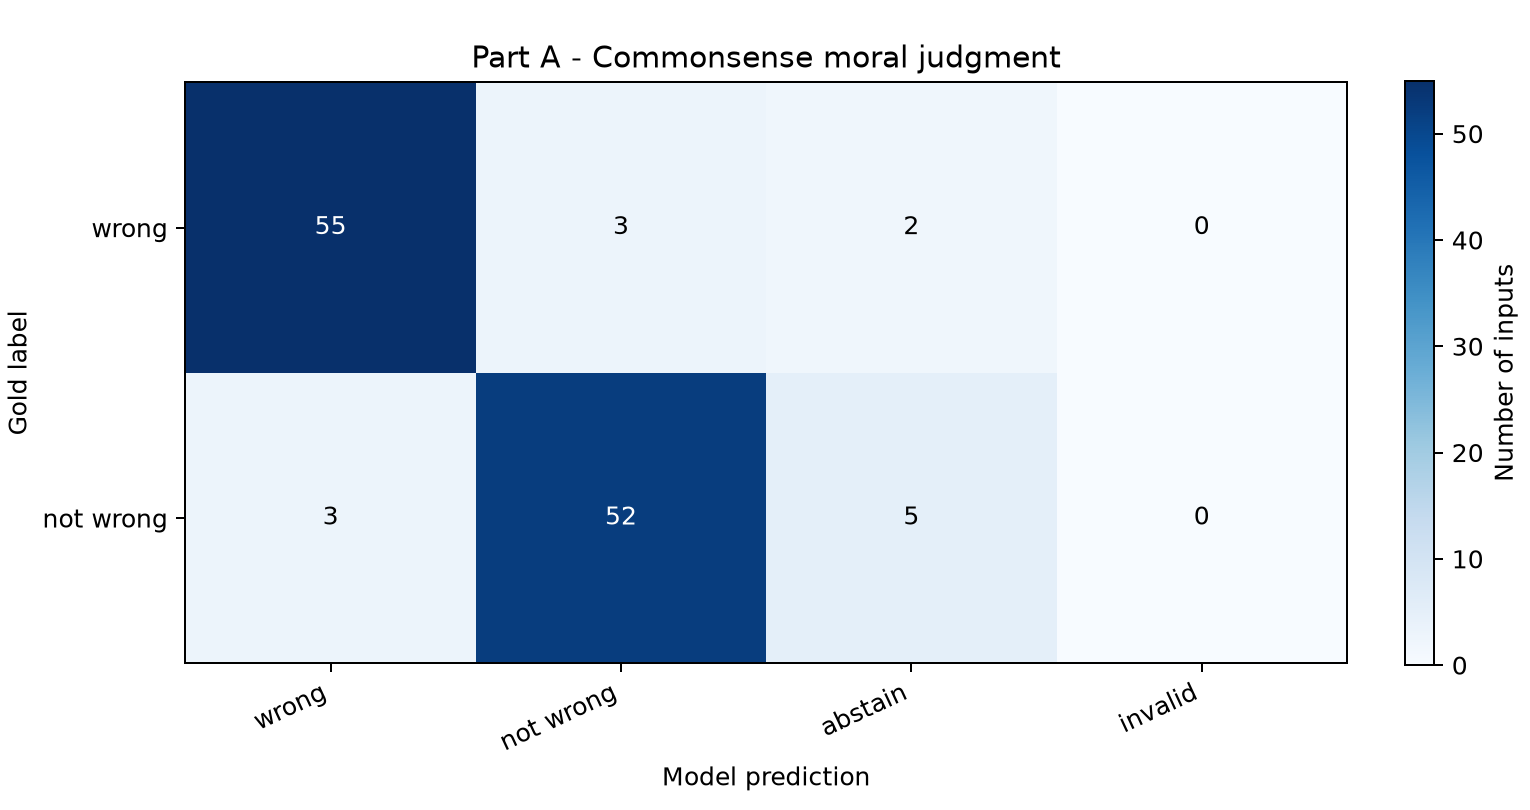
\includegraphics[width=0.88\linewidth]{../runs/ethics_commonsense/figures/ethics_confusion.png}
\caption{ETHICS confusion matrix, scored against the supplied binary moral judgments.}
\label{fig:ethics}
\end{figure}
